\documentclass{rjthesis}
\usepackage{booktabs}        % 设置可以使用三线表
\usepackage{amsmath}         % 设置可以引用数学公式
% 定理类环境宏包
\usepackage{amsthm}
\usepackage[table,xcdraw]{xcolor}
% 插图
\usepackage{graphicx}
\usepackage{subfigure}
% 三线表
\usepackage{booktabs}

% 跨页表格
\usepackage{longtable}

% 算法
\usepackage[linesnumbered,ruled,vlined]{algorithm2e}

% SI 量和单位
\usepackage{siunitx}
\usepackage{svg}
% 参考文献使用 BibTeX + natbib 宏包
% 顺序编码制
% HFUT学位论文样例 参考文献的著录格式

\usepackage[sort]{natbib}
\bibliographystyle{gbt7714-numerical}
% \bibliographystyle{hfutthesis-numerical}
% \bibliographystyle{unsrtnat}
% 配置图片的默认目录
\graphicspath{{figures/}}

% 数学命令
\makeatletter
\newcommand\dif{%  % 微分符号
  \mathop{}\!%
  \ifhfut@math@style@TeX
    d%
  \else
    \mathrm{d}%
  \fi
}
\makeatother
\newcommand\eu{{\symup{e}}}
\newcommand\iu{{\symup{i}}}

% 用于写文档的命令
\DeclareRobustCommand\cs[1]{\texttt{\char`\\#1}}
\DeclareRobustCommand\pkg{\textsf}
\DeclareRobustCommand\file{\nolinkurl}

% hyperref 宏包在最后调用
\usepackage{hyperref}

\rjhead{吴靖宇\hspace{1em}等:静态软件缺陷预测方法研究}

\rjtitle{静态软件缺陷预测方法\textsuperscript{*}}
\rjauthor{吴靖宇}
\rjinfor{\textsuperscript{1}(中国科学技术大学 安徽省计算几何与感知智能重点实验室,安徽 合肥  226019)\\
	
	通讯作者: 吴靖宇, E-mail: andyng@mail.ustc.edu.cn
}

\begin{document}
	
	\rjmaketitle
	\begin{rjabstract}
		近年来,随着随着市场对于高质量游戏场景,高精度三维模型的实时渲染要求,对于高性能图形流水线的需求也越来越多,传统的基于纯硬件的渲染管线面临着巨大的挑战。针对以上问题,本文调研并改进了一种基于分块的软件光栅流水线——CUDARaster。该流水线可以在保持图元顺序的基础上,通过流水线每一个阶段启动特定的CUDA核函数进行光栅化;该流水线支持多种渲染模式,并且实现了一套完整的性能测量体系,方便系统性能测量和优化。
  
  但是该管线年代久远,流水线依赖于底层优化,与其最初设计的GPU架构紧密耦合,无法在现代的GPU架构上充分发挥硬件性能。同时为了保障光栅化计算精度,限制了渲染分辨率。同时,图元保序设计极大的影响了系统性能的进一步扩展。
  
  本次研究的主要工作在探究系统在现代GPU上如何充分发挥性能,故主要工作可分为以下几点:实现线程安全的warp原语,以实现在现代GPU架构上的正确渲染;调研系统的栅格化算法以及限制分辨率的主要原因,并在此基础上实现基于CPU调度的4K分辨率渲染算法;以及为了探究系统性能随Bin block数增加的变化,而实现的改进的规约算法。在此基础之上,我们实现了一个基于分块的软件光栅化渲染器。通过以上改进,提高系统实际应用能力以及可扩展性,为后续的大规模并行渲染系统设计和改进奠定了基础。

	\end{rjabstract}
	\rjkeywords{GPU; 软件光栅化; 并行渲染; CUDA; 分块渲染; 图形管线}

	\section{绪论}

\subsection{研究背景}
图形流水线是一种将三维场景描述输出为二维图像的计算系统,是渲染器的重要组成部分。随着市场对于高质量游戏场景,高精度三维模型的实时渲染要求,对于高性能图形流水线的需求也越来越多。例如,在游戏中,图形流水线可以用于生成动态的光照、阴影和反射,增强游戏的画面质量,为玩家提供视觉享受。在CAD中,基于图形流水线的可视化模块,可以用于渲染高精度的三角网格模型,从而提高设计师的工作效率,保证产品的设计质量。

以著名开源CAD引擎Open CASCAD\cite{opencascad}为例,可视化(渲染)模块是构成CAD引擎的核心之一,不仅对模型的渲染精度提出了要求,还需要满足与设计人员实时交互的需求\cite{cad2023,tvcg18}。

\begin{figure}[tbph]
	\centering
	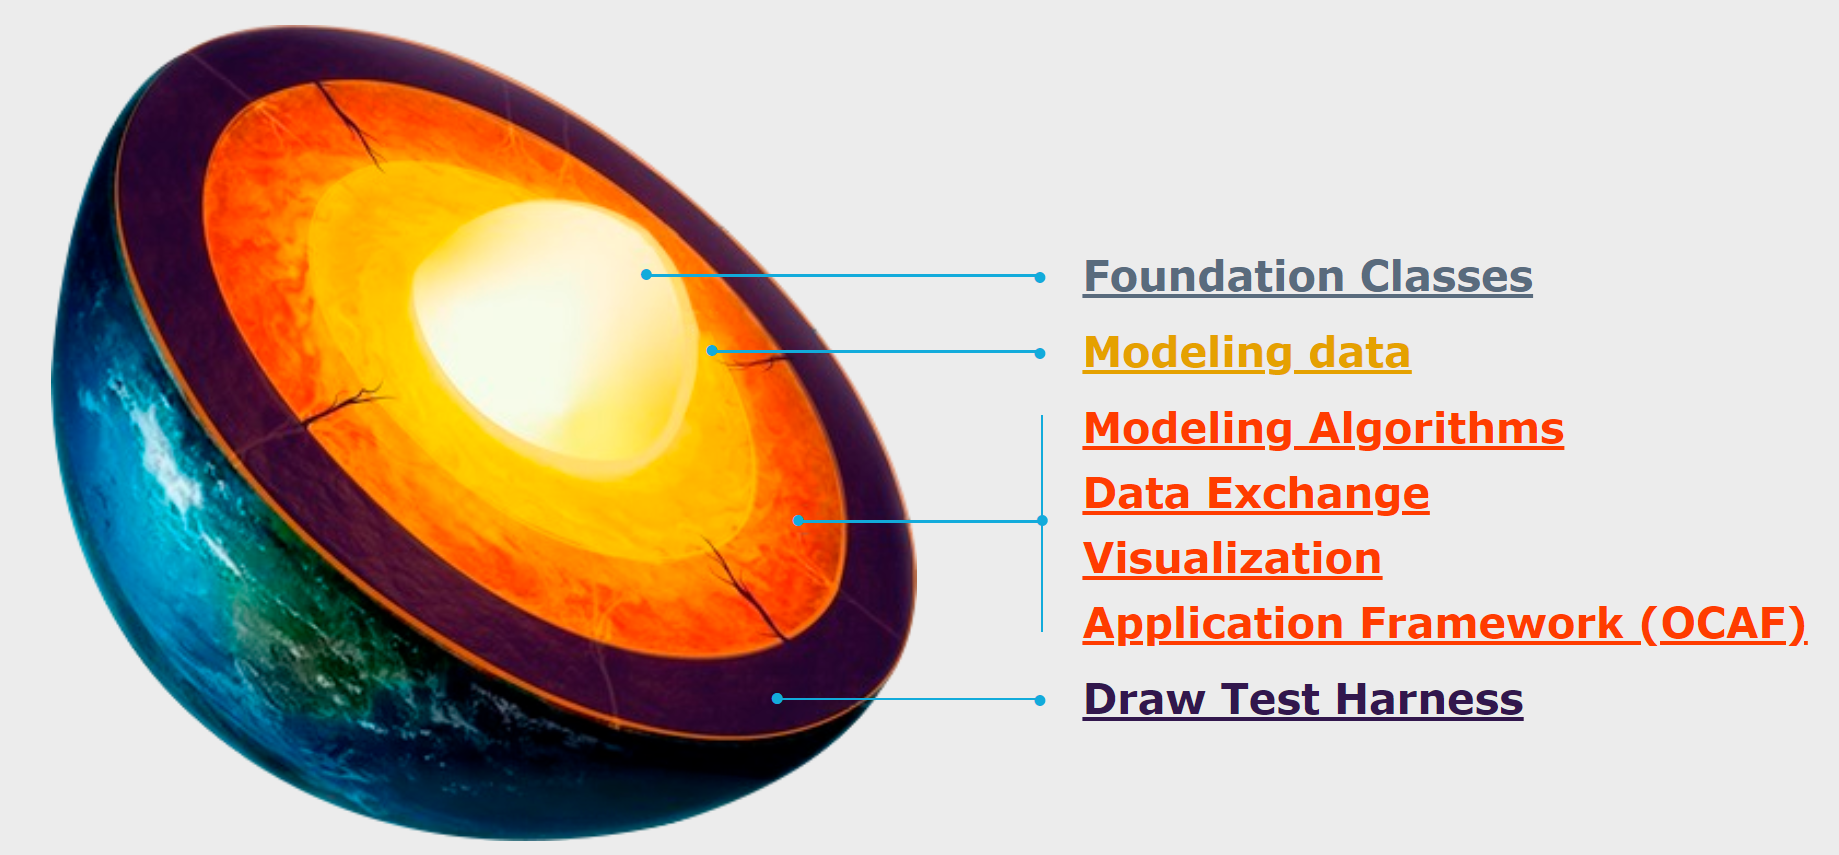
\includegraphics[width=0.8\linewidth]{figures/opencascad}
	\caption[Open CASCAD 系统架构图]{Open CASCAD 系统架构图\cite{opencascad}}
	\label{fig:opencascad}
\end{figure}

	\bibliography{bib/hfut}  % 参考文献使用 BibTeX 编译
	\end{document}